\chapter{Noise, Decoherence and Quantum Error Correction}\label{ch:noise}
\begin{center}\small\textit{Quantum states are fragile. Protecting them is what makes scalable quantum computing possible.}\end{center}

\section{Intuition: Why Quantum Is Fragile}
A classical bit stored as a voltage is robust: small noise does not flip $0$ to $1$ if thresholds are wide. A qubit stores information in continuous amplitudes $\alpha,\beta$ and relative phases. Any stray magnetic field, thermal photon, or crosstalk is a tiny unintended rotation. Because amplitudes are continuous, every imperfection matters, and entanglement with the environment looks like \emph{decoherence} --- the state becomes mixed and interference dies.

Error correction must fight continuous errors with discrete codes. The surprise: it is possible.

\section{Decoherence and Noise Models}
A pure state $\lvert\psi\rangle$ under noise becomes a density matrix $\rho=\sum_i p_i\lvert\psi_i\rangle\langle\psi_i\rvert$. Common channels:

\begin{center}
\begin{tikzpicture}[scale=0.90,font=\footnotesize]
  \fill[blue!10] (0,0) rectangle (3.2,1.6);
  \fill[orange!10] (3.6,0) rectangle (6.8,1.6);
  \fill[green!10] (7.2,0) rectangle (10.4,1.6);
  \draw[thick] (0,0) rectangle (3.2,1.6);
  \draw[thick] (3.6,0) rectangle (6.8,1.6);
  \draw[thick] (7.2,0) rectangle (10.4,1.6);
  \node[font=\scriptsize] at (1.6,1.25) {Bit flip $\mathcal{E}_p$};
  \node[font=\tiny, align=center] at (1.6,0.75) {$X$ with prob.\ $p$\\$\rho\to(1-p)\rho+pX\rho X$};
  \node[font=\scriptsize] at (5.2,1.25) {Phase flip};
  \node[font=\tiny, align=center] at (5.2,0.75) {$Z$ with prob.\ $p$\\kills coherence};
  \node[font=\scriptsize] at (8.8,1.25) {Depolarizing};
  \node[font=\tiny, align=center] at (8.8,0.75) {$X,Y,Z$ each $p/3$\\$\rho\to(1-p)\rho+\tfrac p3\sum P\rho P$};
  \node[fill=violet!10, draw=violet!40!black, rounded corners, inner sep=2pt, font=\tiny] at (5.2,-0.45) {Any single-qubit channel is a mixture of Pauli errors (discretization)};
\end{tikzpicture}
\end{center}

Bloch sphere picture: bit flip shrinks $y$--$z$, phase flip shrinks $x$--$y$, depolarizing shrinks uniformly by $1-p$.

\begin{center}
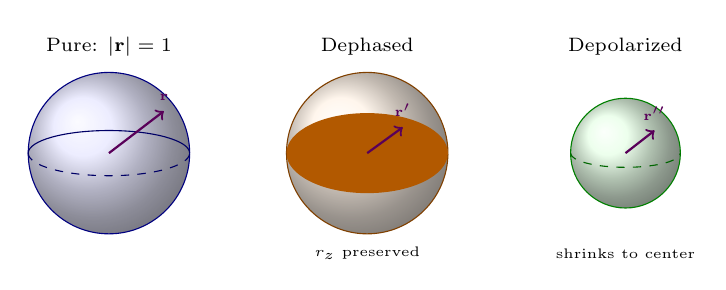
\begin{tikzpicture}[scale=0.82,font=\footnotesize]
  % Pure sphere
  \shade[ball color=blue!12, opacity=0.8] (0,0) circle (1.25);
  \draw[blue!50!black] (0,0) circle (1.25);
  \draw[blue!40!black, dashed] (-1.25,0) arc (180:360:1.25 and 0.35);
  \draw[blue!40!black] (-1.25,0) arc (180:0:1.25 and 0.35);
  \draw[->, thick, violet!70!black] (0,0)--(0.85,0.65) node[above, font=\tiny] {$\mathbf{r}$};
  \node[font=\scriptsize] at (0,1.65) {Pure: $|\mathbf{r}|=1$};
  % Dephased
  \begin{scope}[shift={(4.0,0)}]
    \shade[ball color=orange!12, opacity=0.8] (0,0) circle (1.25);
    \draw[orange!50!black] (0,0) circle (1.25);
    \draw[orange!40!black, dashed] (-1.25,0) arc (180:360:1.25 and 0.35);
    \fill[orange!70!black] (0,0) ellipse (1.25 and 0.62);
    \draw[->, thick, violet!70!black] (0,0)--(0.55,0.4) node[above, font=\tiny] {$\mathbf{r}'$};
    \node[font=\scriptsize] at (0,1.65) {Dephased};
    \node[font=\tiny, fill=white, inner sep=1pt] at (0,-1.55) {$r_z$ preserved};
  \end{scope}
  % Depolarized
  \begin{scope}[shift={(8.0,0)}]
    \shade[ball color=green!12, opacity=0.8] (0,0) circle (0.85);
    \draw[green!50!black] (0,0) circle (0.85);
    \draw[green!40!black, dashed] (-0.85,0) arc (180:360:0.85 and 0.22);
    \draw[->, thick, violet!70!black] (0,0)--(0.45,0.35) node[above, font=\tiny] {$\mathbf{r}''$};
    \node[font=\scriptsize] at (0,1.65) {Depolarized};
    \node[font=\tiny, fill=white, inner sep=1pt] at (0,-1.55) {shrinks to center};
  \end{scope}
\end{tikzpicture}
\end{center}

$T_1$ (relaxation) is amplitude damping $\lvert1\rangle\to\lvert0\rangle$; $T_2$ (dephasing) is loss of phase with $1/T_2=1/2T_1+1/T_\phi$.

\section{Three-Qubit Codes}
Classical repetition $0\to000$, $1\to111$ corrects one bit flip by majority vote. Quantumly we must not measure the data.

\begin{definition}[3-qubit bit-flip code]
$\lvert0_L\rangle=\lvert000\rangle$, $\lvert1_L\rangle=\lvert111\rangle$. Encoding: CNOT$_{0\to1}$, CNOT$_{0\to2}$. Syndrome uses ancilla parity without collapsing $\alpha\lvert0_L\rangle+\beta\lvert1_L\rangle$.
\end{definition}

Syndrome table (ancilla $s_1=Z_0Z_1$, $s_2=Z_1Z_2$): $00$ no error, $10$ flip on qubit 0, $11$ on qubit 1, $01$ on qubit 2. Correction is conditional $X$. Phase-flip code is the same in $H$ basis: $\lvert\pm_L\rangle=\lvert\pm\pm\pm\rangle$.

Shor's 9-qubit code concatenates both: corrects any single-qubit error. In general, discretizing errors: correcting $X$ and $Z$ suffices to correct any $aI+bX+cY+dZ$.

\begin{center}
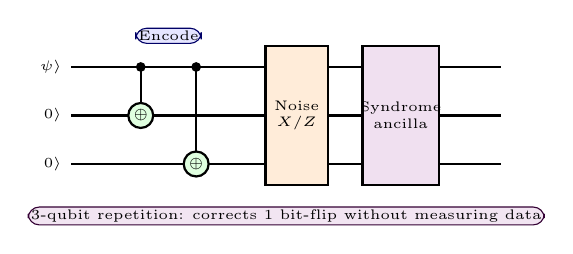
\begin{tikzpicture}[scale=0.88,font=\footnotesize]
  \draw[thick] (0,1.0)--(6.2,1.0);
  \draw[thick] (0,0.3)--(6.2,0.3);
  \draw[thick] (0,-0.4)--(6.2,-0.4);
  \node[left, font=\tiny] at (0,1.0) {$\lvert\psi\rangle$};
  \node[left, font=\tiny] at (0,0.3) {$\lvert0\rangle$};
  \node[left, font=\tiny] at (0,-0.4) {$\lvert0\rangle$};
  \draw[thick] (1.0,1.0)--(1.0,0.3); \fill (1.0,1.0) circle (2pt);
  \draw[thick, fill=green!12] (1.0,0.3) circle (0.18) node[font=\tiny] {$\oplus$};
  \draw[thick] (1.8,1.0)--(1.8,-0.4); \fill (1.8,1.0) circle (2pt);
  \draw[thick, fill=green!12] (1.8,-0.4) circle (0.18) node[font=\tiny] {$\oplus$};
  \node[font=\tiny, fill=blue!10, draw=blue!40!black, rounded corners, inner sep=1pt] at (1.4,1.45) {Encode};
  % Noise
  \draw[fill=orange!15, thick] (2.8,-0.7) rectangle (3.7,1.3) node[midway, align=center, font=\tiny] {Noise\\{\tiny $X$/$Z$}};
  % Syndrome
  \draw[fill=violet!12, thick] (4.2,-0.7) rectangle (5.3,1.3) node[midway, align=center, font=\tiny] {Syndrome\\{\tiny ancilla}};
  \node[font=\tiny, fill=violet!10, draw=violet!40!black, rounded corners, inner sep=1pt] at (3.1,-1.15) {3-qubit repetition: corrects 1 bit-flip without measuring data};
\end{tikzpicture}
\end{center}

\section{Surface Code and Threshold}

\begin{theorem}[Threshold theorem]
If physical error per gate $<p_{\text{th}}\approx10^{-2}$ (surface code $\sim1\%$), concatenating codes suppresses logical error $\epsilon_L\sim(p/p_{\text{th}})^{d/2}$ with code distance $d$, using $\mathrm{polylog}(1/\epsilon)$ overhead. Fault-tolerance is possible.
\end{theorem}

Surface code arranges qubits on a 2-D lattice; $X$ and $Z$ stabilizers are local plaquette checks. Distance $d$ needs $O(d^2)$ physical qubits per logical qubit. Current devices ($50$--$400$ physical qubits, error $\sim10^{-3}$) are below threshold but not yet at large $d$.

\begin{center}
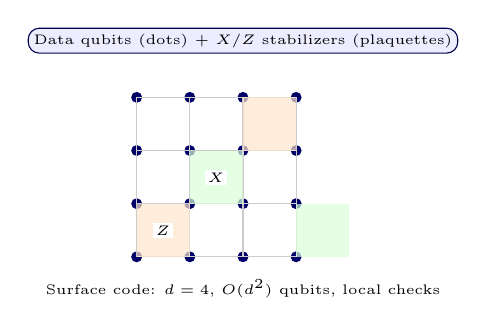
\begin{tikzpicture}[scale=0.90,font=\footnotesize]
  % Surface code lattice 4x4
  \foreach \x in {0,1,2,3} \foreach \y in {0,1,2,3} {
    \fill[blue!40!black] (\x*0.75,\y*0.75) circle (2.2pt);
  }
  \foreach \x in {0,1,2} \foreach \y in {0,1,2} {
    \draw[gray!40] (\x*0.75,\y*0.75) rectangle (\x*0.75+0.75,\y*0.75+0.75);
  }
  % Plaquettes colored
  \fill[orange!20, opacity=0.7] (0,0) rectangle (0.75,0.75);
  \fill[green!15, opacity=0.7] (0.75,0.75) rectangle (1.5,1.5);
  \fill[orange!20, opacity=0.7] (1.5,1.5) rectangle (2.25,2.25);
  \fill[green!15, opacity=0.7] (2.25,0) rectangle (3.0,0.75);
  \node[font=\tiny, fill=white, inner sep=1pt] at (0.37,0.37) {$Z$};
  \node[font=\tiny, fill=white, inner sep=1pt] at (1.12,1.12) {$X$};
  \node[font=\tiny] at (1.5,-0.45) {Surface code: $d=4$, $O(d^2)$ qubits, local checks};
  \node[font=\tiny, fill=blue!7, draw=blue!30!black, rounded corners, inner sep=2pt] at (1.5,3.05) {Data qubits (dots) + $X$/$Z$ stabilizers (plaquettes)};
\end{tikzpicture}
\end{center}

\section{Python: Noise and Repetition Code}

\begin{lstlisting}[language=Python]
import numpy as np

def bitflip_channel(rho, p):
    X = np.array([[0,1],[1,0]], dtype=complex)
    return (1-p)*rho + p*(X @ rho @ X)

def depolarizing(rho, p):
    X = np.array([[0,1],[1,0]], complex)
    Y = np.array([[0,-1j],[1j,0]], complex)
    Z = np.array([[1,0],[0,-1]], complex)
    return (1-p)*rho + p/3*(X@rho@X + Y@rho@Y + Z@rho@Z)

# Bloch shrink demo
plus = np.array([[0.5,0.5],[0.5,0.5]], dtype=complex)  # |+><+|
for p in [0, 0.1, 0.3]:
    r = depolarizing(plus, p)
    # Bloch x = Tr(X rho)
    X = np.array([[0,1],[1,0]], complex)
    print(f"p={p}  <X>={np.trace(X@r).real:.3f} (was 1.0)")

# 3-qubit bit-flip correction
def encode3(psi):  # psi=[a,b] -> a|000>+b|111>
    a,b = psi
    v = np.zeros(8, dtype=complex); v[0]=a; v[7]=b
    return v
\end{lstlisting}

\begin{lstlisting}[language=Python]
# Full 3-qubit syndrome demo
import random

def syndrome_decode(state_vec):
    """Return syndrome bits for single X error model."""
    # parity Z0Z1, Z1Z2: measure without collapsing logical
    probs = np.abs(state_vec)**2
    # simplified: find which basis state dominates
    idx = int(np.argmax(probs))
    bits = format(idx, '03b')
    # syndrome from bits: s1=b0 xor b1, s2=b1 xor b2
    b = [int(c) for c in bits]
    s1, s2 = b[0]^b[1], b[1]^b[2]
    return (s1, s2), bits

psi = [1/np.sqrt(2), 1/np.sqrt(2)]
code = encode3(psi)
print("Encoded |+_L> probs:", np.abs(code)**2)
# Simulate X error on qubit 1 (middle)
X1 = np.kron(np.kron(np.eye(2), np.array([[0,1],[1,0]])), np.eye(2))
err_state = X1 @ code
print("After X1 syndrome:", syndrome_decode(err_state))
# Correction would apply X1 again
recovered = X1 @ err_state
print("Recovered fidelity:", abs(np.vdot(code, recovered))**2)
\end{lstlisting}


\section{Stabilizer Formalism in Brief}
The surface code is a stabilizer code: code space is $+1$ eigenspace of commuting Pauli checks $\{S_i\}$. Measuring $S_i$ gives syndrome without disturbing logical information. Logical operators are strings connecting boundaries, distance is minimal weight of non-trivial logical. Decoding (minimum-weight matching) pairs syndrome defects to infer error. This structure extends to color codes, LDPC codes, and recent good qLDPC advances reducing overhead from $O(d^2)$ toward $O(1)$.

\section{Exercises}
\begin{exercise}
Show bit-flip channel shrinks Bloch vector as $(x,y,z)\to((1-2p)x,(1-2p)y,(1-2p)z)$ for depolarizing? Derive the $T_1\to\infty$ dephasing map $(x,y,z)\to((1-2p)x,(1-2p)y,z)$.
\end{exercise}
\begin{exercise}
Encode $\lvert\psi\rangle=\alpha\lvert0\rangle+\beta\lvert1\rangle$ into $3$-qubit code and list the 4 orthogonal subspaces for no error / $X_0$ / $X_1$ / $X_2$. Why can syndrome be measured without learning $\alpha,\beta$?
\end{exercise}
\begin{exercise}
Construct the $3$-qubit phase-flip code: how does $H^{\otimes3}$ relate it to the bit-flip code? What syndromes detect $Z$ errors?
\end{exercise}
\begin{exercise}
For surface code distance $d=5$ with $p=10^{-3}$, $p_{\text{th}}=10^{-2}$, estimate logical error $\sim(p/p_{\text{th}})^{(d+1)/2}$. How large must $d$ be for $\epsilon_L<10^{-12}$?
\end{exercise}
\begin{exercise}
Simulate amplitude damping with Kraus operators $E_0=\mathrm{diag}(1,\sqrt{1-\gamma})$, $E_1=\sqrt\gamma\lvert0\rangle\langle1\rvert$. Compute Bloch evolution and show it is not unital.
\end{exercise}
